\documentclass[a4paper]{article}
\usepackage[UTF8]{ctex}
\usepackage{geometry}
\usepackage{graphicx}
\usepackage{url}
\usepackage{multirow}
\usepackage{array}
\usepackage{booktabs}
\usepackage{url}
\usepackage{enumitem}
\usepackage{graphicx}
\usepackage{float}
\usepackage{amssymb}
\usepackage{amsmath}
\usepackage{subfig}
\usepackage{longtable}
\usepackage{pifont}
\usepackage{color}

\allowdisplaybreaks

\geometry{a4paper, scale=0.78}

% \begin{figure}[H]
%     \centering
%     \includegraphics[width=.55\textwidth]{E.png}
%     \caption{矩阵与列向量的乘法}
%     \label{fig:my_label_1}
% \end{figure}

% \left\{
% \begin{array}{ll}
%       x+2x+z=2 & \\
%       3x+8y+z=12 & \\
%       4y+z=2
% \end{array}
% \right.

% \begin{enumerate}[itemindent = 1em, itemsep = 0.4pt, parsep=0.5pt, topsep = 0.5pt]

% \end{enumerate}

%\stackrel{a}{\longrightarrow}

\title{Gaussian Process 01 Introduction}
\author{Chen Gong}
\date{13 December 2019}

\begin{document}
\maketitle
本小节我们将进入Gaussian Process的学习。Gaussian自然指的就是Gaussian Distribution,而Process指的就是随机过程。在一维的Gaussian Distribution中我们可以令$p(x) = \mathcal{N}(\mu,\sigma^2)$。如果对应到高维高斯分布的话,也就是(Multivariate Gaussian Distribution)也就是我们通常意义上说的Gaussian Network,对于任意的$x\in \mathbb{R}^p$,有$p(x) = \mathcal{N}(\mu,\Sigma)$,且$\Sigma$是一个$p\times p$维的向量,$p< +\infty$。如果是一个无限维的Gaussian Distribution,那么就是我们今天要讨论的Gaussian Process了。首先我们给出Gaussian Process的详细定义,{\color{red}Gaussian Process:定义在连续域上的无限多个高维随机变量所组成的随机过程。 }所谓连续域指的就是时间或者空间。下面我们来进行详细的解释。

\section{Gaussian Process解释}
我们假设有一组随机变量$\{ \xi_t \}_{t\in T}$,$T$是一个连续域,如果$\forall n \in N^+$,都有$t_1,t_2,\cdots,t_n \in T$,并且存在一个约束条件$s.t.\ \{\xi_{t_1},\xi_{t_2},\cdots,\xi_{t_n}\} \stackrel{\triangle}{=} \xi_{t_1\sim t_n} \sim \mathcal{N}(\mu_{t_1\sim t_n},\Sigma_{t_1\sim t_n})$。那么我们就称$\{ \xi_t \}_{t\in T}$是一个Gaussian Process。那么,我们怎么来通俗的理解这个概念呢?也就是说有一系列在时间上或空间上连续的点,他们之间分开看都是符合一个高斯分布的,而合起来看则是符合一个多维高斯分布的。也就是如下图所示的,在五个不同的时刻有5个不同的点,之上的随机变量为$\{\xi_{t_1},\xi_{t_2},\xi_{t_3},\xi_{t_4},\xi_{t_5}\}$,他们分别都符合一个高斯分布。
\begin{figure}[H]
    \centering
    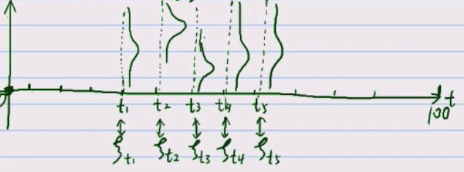
\includegraphics[width=.55\textwidth]{微信图片_20191213121553.png}
    \caption{多个点符合高斯分布的情况}
    \label{fig:my_label_1}
\end{figure}

\section{Gaussian Process举例说明}
为了帮助大家更好的来理解高斯分布,我们在这里讲一个故事。假如一个人的一生可以活到100岁,横坐标就为时间$t$,而纵坐标表示的为在这个时间点的表现值。(大概就这样将就的理解一下)。其中,$t \in [0,100]$,每一个$\xi_t \sim \mathcal{N}(\mu_t,\sigma_t)$。这是什么意思,也就是在每一个时刻这个人的表现值都符合一个独立的高斯分布,也就是在$t$时刻他的表现为$[0,100]$。

现在,我们做一个假设,假设一个人,当$t=0$的时刻,他的一生就已经确定了,也就是他的每一个时刻的表现值都会符合一个确定的Gaussian Distribution,$\mu_t$和$\sigma_t^2$都是确定的。假设人可以活很多次,每个点的表现值都是一个高斯分布,那么他每一生都将是不一样的,没过一生都是从高斯过程中的一次采样,如下图所示,
\begin{figure}[H]
    \centering
    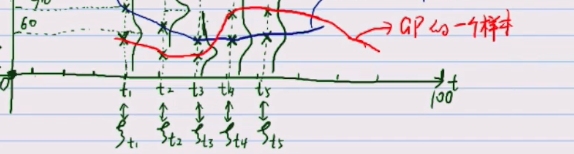
\includegraphics[width=.75\textwidth]{微信图片_20191213130727.png}
    \caption{高斯过程的样本}
    \label{fig:my_label_1}
\end{figure}

所以,$\{\xi_{t_1},\xi_{t_2},\cdots,\xi_{t_n}\}$,本身就是一个高斯分布,他们联合起来也是高斯分布,任何一个采样都属于高斯分布,我们可以看成是高斯过程的一个样本。用符号的语言描述就是$GP(m(t),k(s,t))$。其中
\begin{gather}
    m_t = \mathbb{E}[\xi_t] = mean\ function \\
    k(s,t) = covariance function =\mathbb{E}\left[[\xi_s - m(s)][\xi_t - m(t)]^T\right]
\end{gather}

也就是说,一个高斯过程属于一个多维高斯分布,服从分布的形式为$\mathcal{N}(m_t,k(s,t))$。                                                                                                                                              



\end{document}
